\documentclass[border={0.1cm 0.1cm 0.1cm 0.1cm}]{standalone}  %E,S,W,N

\usepackage{amssymb}
\usepackage{amsmath}
\usepackage{tikz}
\usetikzlibrary{decorations.pathreplacing}	%for brackets

\begin{document}
	
	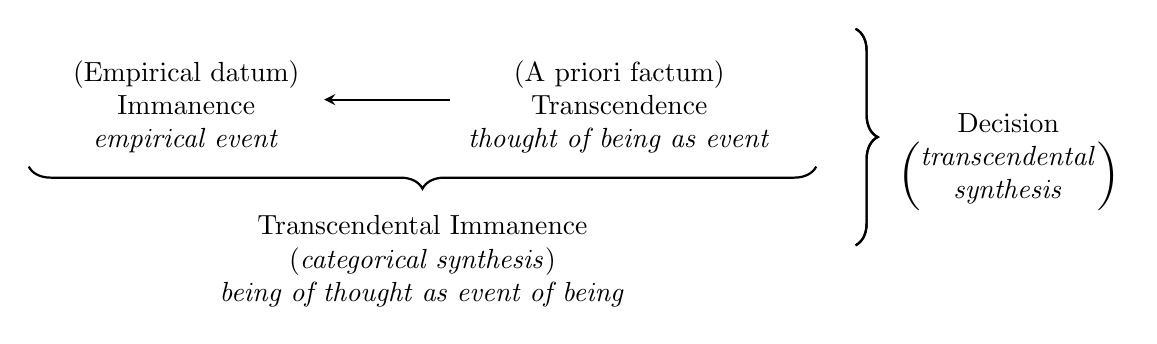
\begin{tikzpicture}	
	\node[align=center,above] at (-3,0.55) {
		(Empirical datum)\\
		Immanence\\
		\textit{empirical event}
	};
	
	\draw[thick,->,>=stealth] (0.35,1.35)--(-1.25,1.35);
	
	\node[align=center,above] at (2.5,0.55) {
		(A priori factum)\\
		Transcendence\\
		\textit{thought of being as event}
	};
	
	\draw[decorate,decoration={brace,amplitude=8pt},thick] (5,0.5)--(-5,0.5);
	
	\node[align=center,below] at (0,0) {
	Transcendental Immanence\\
	(\textit{categorical synthesis})\\
	\textit{being of thought as event of being}
	};
		
	\draw[decorate,decoration={brace,amplitude=8pt},thick] (5.5,2.25)--(5.5,-0.5);
	\draw[decorate,decoration={brace,amplitude=8pt},thick] (5.5,2.25)--(5.5,-0.5);
	
	\node[align=center,right] at (6.2,0.6) {
		Decision\\
		\textit{transcendental}\\
		\textit{synthesis}
	};
	
	\node at (7.45,0.375) {\Huge (\hspace{2.2cm})};
	\end{tikzpicture}
	
\end{document}